\documentclass[format=sigconf]{acmart}
\usepackage[utf8]{inputenc}
\usepackage{geometry}
\usepackage{enumitem}
\usepackage{float}
\usepackage[labelfont=bf,textfont=md]{caption}
\usepackage{graphicx}
\usepackage{svg}
\usepackage{xcolor}
\usepackage{minted}
\usepackage{hyperref}
\usepackage[parfill]{parskip}
\usepackage[all]{hypcap}
\usemintedstyle[common-lisp]{default}
\newmintinline[code]{text}{}
\bibliographystyle{plainnat}

\hypersetup{
  colorlinks,
  linkcolor={red!50!black},
  citecolor={blue!50!black},
  urlcolor={blue!80!black}
}

\newlist{step}{enumerate}{10}
\setlist[step]{label*=\arabic*.,leftmargin=2em}

\acmConference[ELS’25]{the 18th European Lisp Symposium}
{May 19--20 2025}{Zürich, Switzerland}
\acmDOI{10.5281/zenodo.15384117}
\setcopyright{rightsretained}
\copyrightyear{2025}

\begin{document}

\title{Porting the Steel Bank Common Lisp Compiler and Runtime to the Nintendo Switch NX Platform}

\author{Charles Zhang}
\email{charleszhang99@yahoo.com}
\author{Yukari ``Shinmera'' Hafner}
\email{shinmera@tymoon.eu}
\affiliation{%
  \institution{Shirakumo.org}
  \city{Zürich}
  \country{Switzerland}
}

\begin{CCSXML}
<ccs2012>
   <concept>
       <concept_id>10011007.10011006.10011041.10011048</concept_id>
       <concept_desc>Software and its engineering~Runtime environments</concept_desc>
       <concept_significance>500</concept_significance>
       </concept>
   <concept>
       <concept_id>10011007.10011006.10011041.10011045</concept_id>
       <concept_desc>Software and its engineering~Dynamic compilers</concept_desc>
       <concept_significance>500</concept_significance>
       </concept>
   <concept>
       <concept_id>10011007.10010940.10010941.10010949.10010950.10010954</concept_id>
       <concept_desc>Software and its engineering~Garbage collection</concept_desc>
       <concept_significance>300</concept_significance>
       </concept>
   <concept>
       <concept_id>10011007.10011074</concept_id>
       <concept_desc>Software and its engineering~Software creation and management</concept_desc>
       <concept_significance>100</concept_significance>
       </concept>
 </ccs2012>
\end{CCSXML}

\ccsdesc[500]{Software and its engineering~Runtime environments}
\ccsdesc[500]{Software and its engineering~Dynamic compilers}
\ccsdesc[300]{Software and its engineering~Garbage collection}
\ccsdesc[100]{Software and its engineering~Software creation and management}

\begin{abstract}
  We present our efforts to adapt the SBCL runtime and compiler to deploy applications onto the NX platform. The Nintendo Switch (NX) is a 64-bit ARM-based platform for video games with a proprietary micro-kernel operating system. Notably this system does not give programs the ability to mark pages as executable at run time or expose access to thread signal handlers, both of which present a significant hurdle to SBCL's intended bootstrap process and runtime operation. To work around these hurdles we modify SBCL's build system to bootstrap on a Linux ARM system, which is similar enough to the NX to be able to compile user code. We then use a technique called ``shrinkwrapping'' to combine the Lisp code and data with the C runtime compiled for the NX to produce a final, fully static ELF executable that can be run on the NX, without the need for runtime code generation. We further use a restricted version of ``safepoints'' to synchronise threads during garbage collection.
\end{abstract}

\keywords{Common Lisp, SBCL, porting, ARM, aarch64, Nintendo Switch, NX, Experience Report}

\maketitle

\def\abovecaptionskip{1pt}
\def\listingautorefname{Listing}
\def\figureautorefname{Figure}

\begin{figure}[h]
  \centering
  
\includegraphics[width=\linewidth]{switch.jpg}
  \caption{The Nintendo Switch (NX) handheld game console}
\end{figure}

\section{Introduction}\label{introduction}
The Nintendo Switch (codename NX) is a handheld video game console based on the ARM 4 Cortex-A57 64-bit architecture\cite{morgan2020}. It features a proprietary micro-kernel operating system called the ``Nintendo Switch system software''\cite{roussel2019methodically} (NX OS), and normally runs only software that has been licensed, approved, and digitally signed and encrypted by Nintendo.

Developing licensed software for the NX has to be done via Nintendo's own proprietary Software Development Kit (SDK), which they distribute only under a non-disclosure agreement (NDA). An open-source third-party alternative to the SDK is available\cite{switchbrew}, but this cannot be used for licensed software.

The OS-provided runtime environment is directly suitable only for C and C++ software. Other game engines such as Unity, Unreal, and Godot do provide exporting functionality to the NX, meaning that ports for the runtime environments they rely on such as .NET/Mono (C\#), Lua, and GDScript have been developed, but remain closed-source.

Many high-performance native-code Common Lisp implementations operate by compiling and loading user code at runtime into the same process (the state of which is traditionally termed an `image' in the Lisp world). These implementations typically provide a way to dump an image in a way where the runtime of a new process can load it. This implementation technique contrasts with ahead-of-time compilation languages such as C where code is compiled and linked `offline' into an executable whose entire code and runtime gets loaded into its own process by the operating system. On the NX, the SBCL runtime cannot compile and load new code at runtime after an executable is loaded by the operating system on the NX due to platform security restrictions. Because large portions of the system such as the compiler of such image-based Common Lisp implementations are also written in Common Lisp, this restriction means that the implementation must be bootstrapped and all user code compiled ahead of time off of the NX, before the compiled Lisp code in the image can then somehow be linked into a runtime built for the NX by the operating system, rather than relying on the implementation runtime to load the image. We discuss the intricacies of this problem for an image-based implementation such as SBCL in \autoref{build} and \autoref{relocation}.

A port of a Common Lisp implementation such as ECL\cite{attardi1994embeddable}, where Lisp code is compiled to C and easily linked into a C runtime, is conceivable and presents far fewer challenges for building applications for the NX than with an image-based implementation. However, due to the high performance requirements of video games and the relatively low-power platform of the NX, we decided to try and port SBCL, since SBCL produces much faster code than ECL especially with regards to CLOS. In addition, some of the obstacles presented by the NX apply in general to how most Common Lisp implementations function.

For example, the NX OS does not provide user signal handlers. This lack of signal handlers is a problem for the Garbage Collector (GC), as SBCL relies on inter-thread signalling to park threads during garbage collection. While SBCL does provide a safepoints mechanism for GC that is used on Windows which similarly lacks signal handlers, this mechanism is not well tested on other platforms, and as-is still did not meet the requirements of the locked-down NX platform. We discuss the GC in detail in \autoref{gc}.

While we can now compile and deploy complex Common Lisp applications to the NX, some parts of the runtime remain unsupported, and we discuss our future efforts in this regard in \autoref{further-work}.

\section{Related Work}\label{relatedwork}
Rhodes\cite{rhodes2008sbcl} outlines the methodology behind the general SBCL bootstrapping process, which we extend for our locked-down target platform.

A Common Lisp bootstrapping process as Durand et al.\cite{durand2019bootstrapping} outline where the whole target image is created on the host would work to avoid requiring compiling and executing code at runtime on the NX; however, there is not a complete implementation of this technique yet. User libraries which require querying foreign functions at compile time where the details of target architecture matter also cannot be handled with this technique.

Citing information on the operating system of the NX is difficult as it is a closed-source platform with all usual information placed under NDA. All publicly available information is from security research such as by Roussel-Tarbouriech et al.\cite{roussel2019methodically} and reverse-engineering\cite{switchbrew}.

Particularly, we are unaware of any publication about the porting of other runtime environments to the NX, such as C\#, JavaScript, Lua, etc.

Patton\cite{patton2023parallel} and Schwartz\cite{schwartz2018dynamic} describe some details about SBCL's garbage collector which we modify for our port.

\section{Build System}\label{build}
The usual process to build the SBCL compiler and runtime proceeds in several distinct phases, some of which need to be run on a ``host system'' and others on the ``target system''. This process does allow for limited cross-compilation, wherein the ``host system'' steps can be run on an operating system and platform that is not that of the target we are trying to compile for. However, the ``target system'' steps are supposed to run on the target architecture, and involve compiling, loading, and executing new system code in an existing image. As mentioned in the introduction, we cannot load and execute code in the same process that compiled the code on the NX, as the NX OS does not allow us to map new executable pages.

The basic idea of our solution to this issue is to replace the NX as \textit{initial} target with an ARM64-based Linux. Once everything, including user code, has been compiled on this Linux target, we extract all Lisp code and data out using a process called \textit{shrinkwrapping} and link it together with the SBCL C runtime as compiled for the NX. This process ultimately results in a fully static ELF executable that does not perform any dynamic memory mapping or compilation.

Our build still functions largely the same as the one outlined by Rhodes\cite{rhodes2008sbcl}, though being run roughly twice with special configurations to accomplish the hybrid build.

\begin{enumerate}
\item \code{build-config} (NX) \\
  This step gathers whatever build configuration options for the target and spits them out into a readable format for the rest of the build process. We run this on some host system (which may not be our ARM64 Linux intermediary), using a special flag to indicate that we're building for the NX. We also enable the \textit{fasteval} contribution, which we need to step in for any place where we would usually invoke the compiler at runtime.
\item \code{make-host-1} (NX) \\
  Next we build the cross-compiler with the host Lisp compiler, and at the same time emit C header files describing Lisp object layouts in memory as C structs for the next step.
\item \code{make-target-1} (NX) \\
  Now we use the C compiler the Nintendo SDK provides for us, which can cross-compile the SBCL C runtime for the NX. We had to make adjustments to the C runtime bits, as the NX OS is not POSIX compliant and lacks a few features the SBCL C runtime usually takes advantage of. The SBCL C runtime contains the GC and OS glue bits that the Lisp code needs. The artefacts from this stage will later be used in step (10) to attach the C runtime to the shrinkwrapped core.
\item \code{build-config} (Linux$\sim$NX) \\
  We now create an almost-normal ARM64 Linux system with the same feature set as for the NX. This process involves the usual steps as for a ``normal'' Linux ARM64 build, though with a special flag to inform some parts of the Lisp process that we're going to ultimately target the NX.
\item \code{make-host-1} (Linux$\sim$NX) \\
  This step proceeds as usual.
\item \code{make-target-1} (Linux$\sim$NX) \\
  This step proceeds as usual.
\item \code{make-host-2} (Linux$\sim$NX) \\
  With the target runtime built, we build the target Lisp system (compiler and the standard library) using the Lisp cross-compiler built by the Lisp host compiler in \code{make-host-1} (Linux$\sim$NX). This step produces a "cold core" that the runtime can jump into, and can be done purely on the host machine. This cold core is not complete, and needs to be executed on the target machine with the target runtime to finish bootstrapping, notably to initialise the object system, which requires runtime compilation.
\item \code{make-target-2} (Linux$\sim$NX) \\
  The cold core produced in the last step is loaded into the target runtime, and finishes the bootstrapping procedure to compile and load the rest of the Lisp system. After the Lisp system is loaded into memory, the memory is dumped out into a "warm core", which can be loaded back into memory in a new process with the target runtime. From this point on, new code can be loaded and images can be dumped at will.
\item \code{user} \\
  For user code we now perform some tricks to make it think it's running on the NX, rather than on Linux. In particular we modify \code{*features*} to include \code{:nx} and not \code{:linux}, \code{:unix}, or \code{:posix}. Once that is set up and ASDF has been sufficiently tricked into believing we are on the NX, we can compile our program "as usual" and at the end dump out a new core.
\item \code{shrinkwrap} \\
  Once all our code has been loaded and a final core has been produced, we \textit{shrinkwrap} the image to produce assembly files. The details of this technique are outlined in \autoref{relocation}. These assembly files can then be linked together with the SBCL C runtime compiled for the NX in step (3) with the Nintendo SDK toolchain, producing a final ELF executable.
\item \code{package} \\
  The final step is to run all the other SDK toolchain bits to produce a signed application package, which can be deployed to a Nintendo Switch development kit to be run.
\end{enumerate}

\begin{figure}[h]
  \centering
  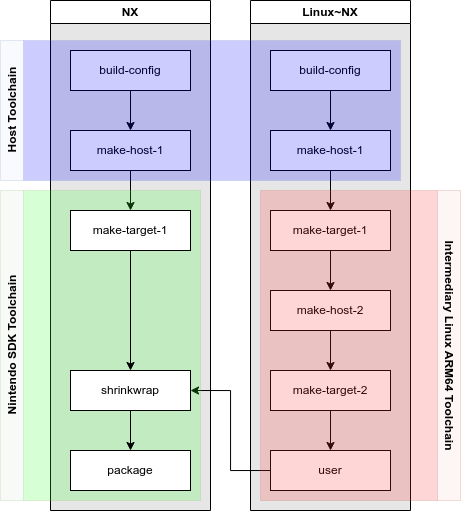
\includegraphics[width=\linewidth]{build.png}
  \caption{A diagram of the build steps and their dependencies}
\end{figure}

A notable extra wrinkle in this procedure is that the SDK is available only for Windows. To accommodate this platform restriction, the custom build system we developed to automate these steps can be run either directly from Windows using another ARM machine remotely to run the Linux bits, or it can be run from a Linux system with the ARM bits being run either locally or remotely and the Windows bits being run either remotely or through Wine\cite{amstadt1994wine}.

\section{Relocation}\label{relocation}
Lisp objects in memory contain absolute pointers, with the result that dumping the in-process state of all Lisp memory spaces to disk results in a \textit{core image} filled with absolute pointers. Traditionally, image-based Lisp implementations such as SBCL map their address spaces to fixed addresses for two reasons: First, reloading an image into a process is easier this way, since objects can be mapped back in the new image directly to where they were in the process that dumped the image. Second, some architecture backends optimize code generation by hardwiring the address of certain Lisp objects directly into the machine code.

\subsection{Address Space Layout Randomization}
Because the NX operating system enforces address space layout randomization, the Lisp runtime cannot rely on being able to map its address spaces to fixed addresses. Hence, the runtime must relocate all objects present in the dumped image to the address spaces placed randomly by the operating system. As part of our work, we have extended the existing support for heap relocation to allow all other Lisp spaces used by SBCL to be relocated as well, with the result being that the runtime can fix up all absolute pointers mapped in from the image to point to the random addresses given to the runtime by the operating system. In addition, we modified the Lisp code generation to produce strictly position-independent code.

However, code objects still present a special problem on the NX for this relocation process. A code object in SBCL is represented like other Lisp objects in-memory, in that it has a header word describing the type and size of code object. The code object also contains slots pointing to the debug information associated with the code object as well as other boxed objects which represent constants referenced by the code instructions. This is so that the garbage collector can scan the code object and fix up these boxed pointers as it does with other Lisp objects. Finally, these slots are followed by the raw machine instructions and function entry points representing the compiled Lisp code. The code object associated with the function defined in \autoref{lst:function} is illustrated in \autoref{fig:before-shrinkwrap}.

\begin{listing}[h]
\begin{minted}[fontsize=\small]{lisp}
(defun f ()
  (cons '(42 . 1958) 'els2025))

\end{minted}
\caption{A Lisp function referencing the constants \code{'(42 . 1958)} and \code{'ELS2025}.}
\label{lst:function}
\end{listing}

Notably, the code object contains both executable machine code and absolute pointers to Lisp objects. Because the machine instructions are to be executed by the CPU, the pages the code object is allocated on must be marked executable by the runtime.

\begin{figure}[h]
  \centering
  \includesvg[width=\linewidth]{Code object before shrinkwrapping.drawio.svg}
  \caption{Representation of the compiled code object (in boldface)
    for the function \protect\texttt{\#'f} in memory, along with the
    cons and symbol objects it references.}
  \label{fig:before-shrinkwrap}
\end{figure}

However, executable pages are not writable on the NX, meaning the pointers to boxed Lisp data for the debug information and code constants cannot be fixed up as part of the relocation process on start-up. Furthermore, only the system loader is able to allocate executable pages by loading code from on-disk ELF .text sections, meaning it isn't possible to first fix up boxed object pointers in the code object \emph{before} marking the code pages executable. In either case, the garbage collector would not be able to fix up these pointers either. Therefore, the code and data need to be separated, at first so that the runtime can relocate the absolute pointers to the Lisp objects, and later so that the moving garbage collector is able to fix up those references. This restriction requires the shrinkwrapping procedure to separate the data from the code and to rewrite the code in the image offline so that any references in code to code constants\footnote{As for the per-code-object slot containing debug information, we modified the Lisp system so that debug information is not accessed through the code object at all but rather through a weak hash table keyed by code object.} are into a dislocated read/write space instead of into the code object itself, which is on an executable page and hence not writable on the NX. To demonstrate this process in more detail, our modified offline shrinkwrapping process produces two artefacts from a normal Lisp image:

\begin{figure}[h]
  \centering
  \includesvg[width=\linewidth]{Code objects in memory after shrinkwrapping.drawio.svg}
  \caption{Representation of the same code object and the cons and
    symbol objects it references after code/data segregation and the
    rest of the shrinkwrapping process.}
  \label{fig:after-shrinkwrap}
\end{figure}

\begin{itemize}
\item \code{pie-shrinkwrap-sbcl.s}: A textual assembly file is generated with all code objects in the original core image listed under \code{.text} sections. The pointers to debug information and code constants inside the code object are zeroed out, and the code constants referenced via the ARMv8 \code{LDR} instruction are displaced into a r/w \code{.data} section shared by all code objects. The \code{LDR} instructions are rewritten to access the constants from this section instead.
\item \code{pie-shrinkwrap-sbcl.o}: A binary object file with the rest of the Lisp data from the core image section is generated. The majority of the Lisp image is thus `shrinkwrapped' into a large r/w \code{.data} section.
\end{itemize}

The reason for producing both a textual and a binary artefact is that it is easier to rewrite and produce textual assembly for code, and it is faster to process and link a binary artefact for the rest of the data. \autoref{fig:after-shrinkwrap} illustrates how the code object for the function \code{#'f} gets split up. The shrinkwrapping process then links both artefacts with the rest of the SBCL runtime to produce the final executable. The upshot of this process is that both the relocation process and the garbage collector can now scan and fix up all boxed pointers in the image at runtime without running into the read-only constraint for executable pages.

\subsection{Linkage between Lisp and foreign code}
Another part of the system impacted by the need for relocation is linkage between Lisp and foreign code. SBCL uses a linkage table that indirects calls to foreign code from Lisp so that foreign code can be loaded by the operating system at any address on startup and resolved in the linkage table. However, for callbacks into Lisp from foreign code, Lisp must create function pointers to snippets of assembly allocated in static (i.e. never moved by GC) Lisp space. These pointers can then be passed to and called from foreign code. To ensure that such function pointers in a saved image are valid even after the Lisp spaces containing the callback entry points are relocated, the function pointers must somehow be fixed up. We managed to solve this problem by having the offline shrinkwrapping process move the callback entry code into another \code{.text} ELF section while recording fixup information. The operating system can then load the callback entry code into executable pages, and the Lisp runtime can rewrite the static function pointers to point to where the code was loaded using the recorded fixup information.

\section{Garbage Collection}\label{gc}
SBCL's default garbage collector, \textit{gencgc}, is a stop-the-world collector, meaning it must stop or \textit{park} other threads in the process. Doing so is necessary so that the threads don't access any memory that the collector might move or change during collection. On RISC architectures like the ARM the Nintendo Switch runs on, the collector is also precise and must be able to identify which storage locations contain Lisp objects, so it is important that the threads are parked at code locations where the collector can safely do so.

In the discussion that follows, a \textit{Lisp thread} is a native thread registered to the Lisp runtime that can either be executing Lisp or foreign code. Native threads created by Lisp are immediately registered to the runtime. A native thread created by foreign code that calls into Lisp via e.g. a callback gets a Lisp thread associated with it by the runtime when it starts executing Lisp code for the first time.

On Unix systems, the POSIX signal mechanism is used by default to park all Lisp threads besides the thread executing GC. By sending a signal to every other thread, each thread will enter a signal handler, which can then park the thread. This method is advantageous, since it leverages an operating system mechanism to interrupt thread execution and frees the thread from checking whether it should park. The garbage collector can also use the signal context mechanism to read and process the values of all registers and the Lisp stack at the point where the thread stopped. On the flip side, Lisp code must be generated in such a way that the GC almost always knows how to parse Lisp objects from registers or the stack at any code location. However, certain instruction sequences in the generated code then need to behave atomically in the sense that it is not safe to stop for GC at those locations, so extra bookkeeping is done to defer interrupts in those sequences. Lisp threads in foreign code are stopped and restarted just as Lisp threads are in Lisp code, though only the contents of its stack are scavenged.

On Windows, no equivalent signal mechanism is available, so a strategy using safepoints must be employed instead. A \textit{safepoint} is a location in code which is known to be GC-safe, so the collector has enough information at that location to correctly function. The Lisp compiler then injects code (here termed \textit{yieldpoint} code) at these safepoints, such as at function call boundaries and loop returns, which causes the thread to check whether it should yield for GC. Yieldpoint code should be inserted strategically so that it doesn't take too long for threads to park after a given thread decides to collect garbage, but also so that the overhead of checking whether to park the thread is as low as possible. Lisp threads in foreign code do not encounter yieldpoint code generated by the GC, but also do not need to be parked anyway, as foreign code is assumed to not access Lisp data. Its Lisp stack can still be safely scavenged while the thread is executing foreign code. However, since the thread is not stopped, it is possible that the thread may re-enter Lisp during a collection, in which case code for re-entry into Lisp must check if GC is running and park the thread and wait for GC to complete before the thread can execute Lisp code again. A similar consideration applies for Lisp threads in Lisp which enter foreign code while the collecting thread is waiting for all Lisp threads in Lisp code to stop; the Lisp thread must communicate to the GC that it is entering foreign code and hence the collecting thread need not wait for it to yield anymore, since the Lisp thread is about to start executing foreign code. For the purposes of this paper, we will call these points of communication at foreign function call boundaries \textit{foreign yieldpoints}.

To summarize, the safepoint and signal mechanisms can be seen as inverses of each other: whereas code generation for the signal mechanism must ensure that the majority of code locations are safe for GC, the safepoint mechanism requires only that strategically chosen locations are safe for GC. The safepoint mechanism also allows foreign code to run without stopping at the cost of extra communication at foreign call boundaries, while the signal mechanism stops all Lisp threads regardless of whether they are executing foreign code or not.

In the existing safepoint ports, SBCL exploits hardware memory protection facilities provided by the operating system in order to make generated yieldpoint code as small as possible: GC toggles the read and write permission bits of pages in virtual memory in order to communicate to the thread various GC state transitions. Non-foreign yieldpoint code then consists of a single read instruction from a global page that a GC marks as non-readable when it wants all Lisp threads to park. The resulting page fault traps into trap handler code that yields the thread and progresses the state of the GC. Foreign yieldpoint code consists of a write instruction onto a thread-local page, informing the GC whether the Lisp thread is entering or leaving foreign code; the GC is then able to selectively cause the relevant threads to trap and wait for the state of the GC to progress or allow the relevant threads to continue toggling the write permissions of the thread-local page accordingly. One other advantage of using page permissions is that it allows race-free examine + wait + use in the latter scenario where the `entry into/return from foreign code' flag word in memory needs to be read and appropriately acted on.

\subsection{Challenges for the NX}
As the NX also does not expose a POSIX signal mechanism, we chose to use the safepoint strategy as a starting point. However, as mentioned previously, even the safepoint strategy relies on hardware memory protection facilities to aid inter-thread communication between the collecting thread and other threads. The NX does not provide ways to install trap handlers for memory faults in release mode, so a different mechanism had to be devised.

For non-foreign yieldpoint code, it sufficed to replace the trapping read instruction with a polling instruction sequence which simply checks if a global `stop now' word is true and if so, branches into a trampoline which calls into the trap handling code. Since there is no hardware trap and associated register context under this scheme, the trampoline also serves to spill all registers onto the Lisp stack so that the garbage collector correctly scavenges and fixes up the roots contained in the registers at the safepoint.

For foreign yieldpoint code, we replace the page permission scheme by designating an additional `permission' word on the thread local page in addition to the `entry into/return from foreign code' flag word to emulate the effect of the page permission scheme: the additional word flags whether write access to the other word is allowed. Since the thread containing the page and the collector thread may both race to access the two words in memory, the code sequence examining the permission word and dispatching to the correct GC state handler based on the value of the flag word requires explicit synchronization primitives. For now, we use locks to ensure race-free communication between the collector thread and any threads which are entering or exiting foreign code.

In addition to the existing safepoint mechanism requiring hardware page protection facilities, the garbage collector also used certain virtual-memory tricks to quickly zero out and/or return large chunks of memory back to the operating system. As the NX does not expose such sophisticated virtual memory management to the application developer, we had to rely on slower and more portable means of achieving the same effect.

\section{Conclusion}\label{conclusion}
We have demonstrated that it is possible to port SBCL even to a very restrictive platform that is hostile towards dynamic runtimes such as used for Lisp.

\begin{figure}[h]
  \centering
  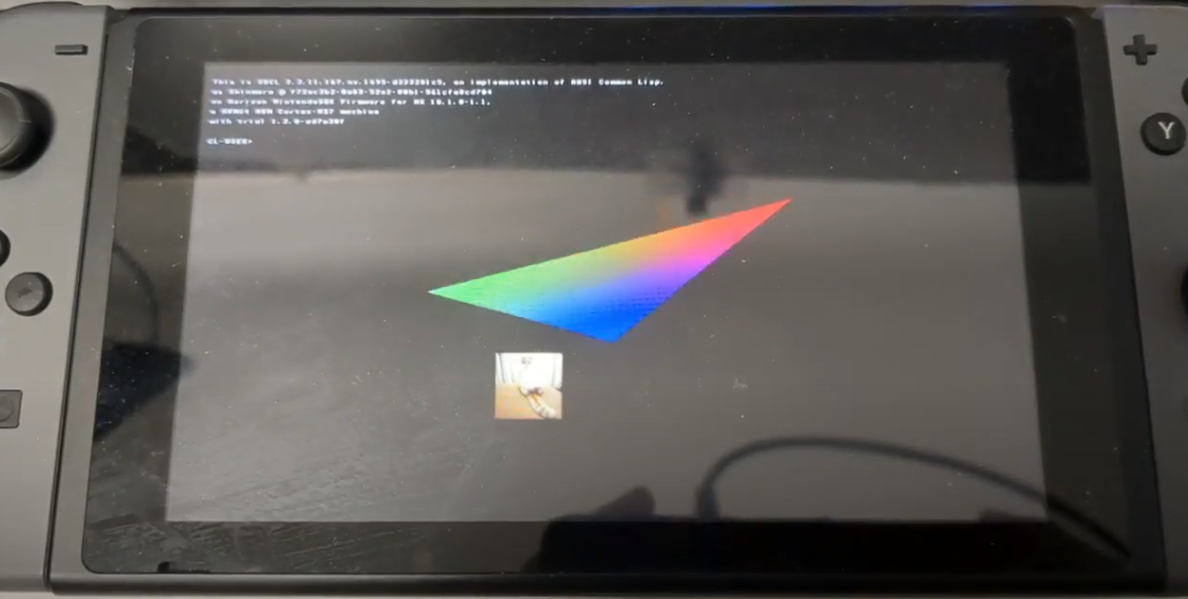
\includegraphics[width=\linewidth]{photo.png}
  \caption{A demo running in the Trial Common Lisp game engine on the Nintendo Switch development hardware}
\end{figure}

Using a substitute build host that is similar enough to the target platform, we can compile all code ahead of time, then substitute the base runtime and rewrite the resulting code in order to create an executable suitable for the target platform.

We have also managed to update the garbage collector to work on operating systems with more restrictive feature sets than are found on a typical desktop operating system.

\section{Further Work}\label{further-work}
Currently, we rely on the \textit{fasteval} system to circumvent runtime compilation restrictions. This is especially vital for CLOS, since the discriminating function is compiled only on first call of a generic function. However, since we know that we don't dynamically add or remove methods, we should be able to pre-compile all of these functions as well. We'd like to add such a CLOS freeze step to the build pipeline, perhaps using a technique similar to \textit{satiation} as outlined by Strandh et al.\cite{strandh2014resolving}

We also unfortunately have not yet had the time to successfully adapt Shirakumo Games' previous title, Kandria, to work on the NX. This port is currently in progress, and it is likely that further minor incompatibilities or bugs in our current SBCL port will surface as part of this effort.

The follow-up console to the Nintendo Switch, called ``Switch 2'' has also recently been announced. The device is backwards compatible with the NX and we expect that the operating environment will be very similar if not identical to that of the NX, just with more RAM and a better CPU and GPU. We hope to receive developer access to the Switch 2 and ensure that the port works for that, too.

Finally there are a number of improvements we've made that we would like to upstream to lessen the maintenance burden. We've already contributed a bunch of the changes back upstream, but a lot of it is also tied to the proprietary SDK and cannot be open-sourced due to the NDA, and some other changes are too contentious for the rest of the SBCL team to want to upstream.

\section{Acknowledgements}\label{acknowledgements}
We would like to thank Douglas Katzman for his help and advice for various parts of the porting effort, as well as the rest of the SBCL maintenance team for their continuous improvements to the SBCL platform. We would also like to thank Robert Strandh and Jan Moringe for their feedback on the draft paper.

\bibliography{paper}

\end{document}

%%% Local Variables:
%%% mode: latex
%%% TeX-command-extra-options: "-shell-escape"
%%% TeX-master: t
%%% TeX-engine: luatex
%%% End:
